
%-----------------------------------------------------------------------------
% PACKAGES AND OTHER DOCUMENT CONFIGURATIONS
%-----------------------------------------------------------------------------

\documentclass[11pt,addpoints,answers]{exam}
\usepackage[margin=1in]{geometry}
\usepackage{amsmath, amsfonts}
\usepackage{enumerate}
\usepackage{graphicx}
\usepackage{titling}
\usepackage{url}
\usepackage{xfrac}
\usepackage{natbib}
\usepackage{amssymb}
\usepackage{amsthm}
\usepackage{paralist}
\usepackage{epstopdf}
\usepackage{tabularx}
\usepackage{longtable}
\usepackage{multirow}
\usepackage{multicol}
\usepackage[colorlinks=true,urlcolor=blue]{hyperref}
\usepackage{algorithm}
\usepackage{algorithmicx}
\usepackage[noend]{algpseudocode}
\usepackage{float}
\usepackage{enumerate}
\usepackage{array}
\usepackage{environ}
\usepackage{times}
\usepackage{textcomp}
\usepackage{caption}
\usepackage{parskip} % For NIPS style paragraphs.
\usepackage[compact]{titlesec} % Less whitespace around titles
\usepackage[inline]{enumitem} % For inline enumerate* and itemize*
\usepackage{datetime}
\usepackage{comment}
% \usepackage{minted}
\usepackage{lastpage}
\usepackage{color}
\usepackage{xcolor}
\usepackage[final]{listings}
\usepackage{tikz}
\usetikzlibrary{shapes,decorations}
\usepackage{framed}
\usepackage{booktabs}
\usepackage{cprotect}
\usepackage{verbatimbox}
\usepackage{multicol}
\usepackage{hyperref}
\usepackage{subcaption}
\usepackage{mathtools} % For drcases
\usepackage{cancel}
\usepackage[many]{tcolorbox}
\usepackage{soul}
\usepackage[bottom]{footmisc}
\usepackage{bm}
\usepackage{wasysym}

\usepackage{tikz}
\usetikzlibrary{shapes.geometric}
\usetikzlibrary{positioning, arrows, automata}

\newtcolorbox[]{your_solution}[1][]{%
    % breakable,
    enhanced,
    nobeforeafter,
    colback=white,
    title=Your Answer,
    sidebyside align=top,
    box align=top,
    #1
}

%%%%%%%%%%%%%%%%%%%%%%%%%%%%%%%%%%%%%%%%%%%
% Rotated Column Headers                  %
%%%%%%%%%%%%%%%%%%%%%%%%%%%%%%%%%%%%%%%%%%%
\usepackage{adjustbox}
\usepackage{array}

%https://tex.stackexchange.com/questions/32683/rotated-column-titles-in-tabular

\newcolumntype{R}[2]{%
    >{\adjustbox{angle=#1,lap=\width-(#2)}\bgroup}%
    l%
    <{\egroup}%
}
\newcommand*\rot{\multicolumn{1}{R{45}{1em}}}% no optional argument here, please!


%%%%%%%%%%%%%%%%%%%%%%%%%%%%%%%%%%%%%%%%%%%
% Better numbering                        %
%%%%%%%%%%%%%%%%%%%%%%%%%%%%%%%%%%%%%%%%%%%

% \numberwithin{equation}{section} % Number equations within sections (i.e. 1.1, 1.2, 2.1, 2.2 instead of 1, 2, 3, 4)
% \numberwithin{figure}{section} % Number figures within sections (i.e. 1.1, 1.2, 2.1, 2.2 instead of 1, 2, 3, 4)
% \numberwithin{table}{section} % Number tables within sections (i.e. 1.1, 1.2, 2.1, 2.2 instead of 1, 2, 3, 4)

%%%%%%%%%%%%%%%%%%%%%%%%%%%%%%%%%%%%%%%%%%
% Custom commands                        %
%%%%%%%%%%%%%%%%%%%%%%%%%%%%%%%%%%%%%%%%%%

\newcommand{\vc}[1]{\boldsymbol{#1}}
\newcommand{\adj}[1]{\frac{d J}{d #1}}
\newcommand{\chain}[2]{\adj{#2} = \adj{#1}\frac{d #1}{d #2}}

\newcommand{\independent}{\perp\!\!\!\perp}

\newcommand{\R}{\mathbb{R}}
\newcommand{\blackcircle}{\tikz\draw[black,fill=black] (0,0) circle (1ex);}
\renewcommand{\circle}{\tikz\draw[black] (0,0) circle (1ex);}

\newcommand{\emptysquare}{{\LARGE $\square$}\ \ }
\newcommand{\filledsquare}{{\LARGE $\boxtimes$}\ \ }
\newcommand{\emptycircle}{{\LARGE $\fullmoon$}\ \ }
\newcommand{\filledcircle}{{\LARGE $\newmoon$}\ \ }


% mathcal
\newcommand{\Ac}{\mathcal{A}}
\newcommand{\Bc}{\mathcal{B}}
\newcommand{\Cc}{\mathcal{C}}
\newcommand{\Dc}{\mathcal{D}}
\newcommand{\Ec}{\mathcal{E}}
\newcommand{\Fc}{\mathcal{F}}
\newcommand{\Gc}{\mathcal{G}}
\newcommand{\Hc}{\mathcal{H}}
\newcommand{\Ic}{\mathcal{I}}
\newcommand{\Jc}{\mathcal{J}}
\newcommand{\Kc}{\mathcal{K}}
\newcommand{\Lc}{\mathcal{L}}
\newcommand{\Mc}{\mathcal{M}}
\newcommand{\Nc}{\mathcal{N}}
\newcommand{\Oc}{\mathcal{O}}
\newcommand{\Pc}{\mathcal{P}}
\newcommand{\Qc}{\mathcal{Q}}
\newcommand{\Rc}{\mathcal{R}}
\newcommand{\Sc}{\mathcal{S}}
\newcommand{\Tc}{\mathcal{T}}
\newcommand{\Uc}{\mathcal{U}}
\newcommand{\Vc}{\mathcal{V}}
\newcommand{\Wc}{\mathcal{W}}
\newcommand{\Xc}{\mathcal{X}}
\newcommand{\Yc}{\mathcal{Y}}
\newcommand{\Zc}{\mathcal{Z}}

% mathbb
\newcommand{\Ab}{\mathbb{A}}
\newcommand{\Bb}{\mathbb{B}}
\newcommand{\Cb}{\mathbb{C}}
\newcommand{\Db}{\mathbb{D}}
\newcommand{\Eb}{\mathbb{E}}
\newcommand{\Fb}{\mathbb{F}}
\newcommand{\Gb}{\mathbb{G}}
\newcommand{\Hb}{\mathbb{H}}
\newcommand{\Ib}{\mathbb{I}}
\newcommand{\Jb}{\mathbb{J}}
\newcommand{\Kb}{\mathbb{K}}
\newcommand{\Lb}{\mathbb{L}}
\newcommand{\Mb}{\mathbb{M}}
\newcommand{\Nb}{\mathbb{N}}
\newcommand{\Ob}{\mathbb{O}}
\newcommand{\Pb}{\mathbb{P}}
\newcommand{\Qb}{\mathbb{Q}}
\newcommand{\Rb}{\mathbb{R}}
\newcommand{\Sb}{\mathbb{S}}
\newcommand{\Tb}{\mathbb{T}}
\newcommand{\Ub}{\mathbb{U}}
\newcommand{\Vb}{\mathbb{V}}
\newcommand{\Wb}{\mathbb{W}}
\newcommand{\Xb}{\mathbb{X}}
\newcommand{\Yb}{\mathbb{Y}}
\newcommand{\Zb}{\mathbb{Z}}

% mathbf lowercase
\newcommand{\av}{\mathbf{a}}
\newcommand{\bv}{\mathbf{b}}
\newcommand{\cv}{\mathbf{c}}
\newcommand{\dv}{\mathbf{d}}
\newcommand{\ev}{\mathbf{e}}
\newcommand{\fv}{\mathbf{f}}
\newcommand{\gv}{\mathbf{g}}
\newcommand{\hv}{\mathbf{h}}
\newcommand{\iv}{\mathbf{i}}
\newcommand{\jv}{\mathbf{j}}
\newcommand{\kv}{\mathbf{k}}
\newcommand{\lv}{\mathbf{l}}
\newcommand{\mv}{\mathbf{m}}
\newcommand{\nv}{\mathbf{n}}
\newcommand{\ov}{\mathbf{o}}
\newcommand{\pv}{\mathbf{p}}
\newcommand{\qv}{\mathbf{q}}
\newcommand{\rv}{\mathbf{r}}
\newcommand{\sv}{\mathbf{s}}
\newcommand{\tv}{\mathbf{t}}
\newcommand{\uv}{\mathbf{u}}
\newcommand{\vv}{\mathbf{v}}
\newcommand{\wv}{\mathbf{w}}
\newcommand{\xv}{\mathbf{x}}
\newcommand{\yv}{\mathbf{y}}
\newcommand{\zv}{\mathbf{z}}

% mathbf uppercase
\newcommand{\Av}{\mathbf{A}}
\newcommand{\Bv}{\mathbf{B}}
\newcommand{\Cv}{\mathbf{C}}
\newcommand{\Dv}{\mathbf{D}}
\newcommand{\Ev}{\mathbf{E}}
\newcommand{\Fv}{\mathbf{F}}
\newcommand{\Gv}{\mathbf{G}}
\newcommand{\Hv}{\mathbf{H}}
\newcommand{\Iv}{\mathbf{I}}
\newcommand{\Jv}{\mathbf{J}}
\newcommand{\Kv}{\mathbf{K}}
\newcommand{\Lv}{\mathbf{L}}
\newcommand{\Mv}{\mathbf{M}}
\newcommand{\Nv}{\mathbf{N}}
\newcommand{\Ov}{\mathbf{O}}
\newcommand{\Pv}{\mathbf{P}}
\newcommand{\Qv}{\mathbf{Q}}
\newcommand{\Rv}{\mathbf{R}}
\newcommand{\Sv}{\mathbf{S}}
\newcommand{\Tv}{\mathbf{T}}
\newcommand{\Uv}{\mathbf{U}}
\newcommand{\Vv}{\mathbf{V}}
\newcommand{\Wv}{\mathbf{W}}
\newcommand{\Xv}{\mathbf{X}}
\newcommand{\Yv}{\mathbf{Y}}
\newcommand{\Zv}{\mathbf{Z}}

% bold greek lowercase
\newcommand{\alphav     }{\boldsymbol \alpha     }
\newcommand{\betav      }{\boldsymbol \beta      }
\newcommand{\gammav     }{\boldsymbol \gamma     }
\newcommand{\deltav     }{\boldsymbol \delta     }
\newcommand{\epsilonv   }{\boldsymbol \epsilon   }
\newcommand{\varepsilonv}{\boldsymbol \varepsilon}
\newcommand{\zetav      }{\boldsymbol \zeta      }
\newcommand{\etav       }{\boldsymbol \eta       }
\newcommand{\thetav     }{\boldsymbol \theta     }
\newcommand{\varthetav  }{\boldsymbol \vartheta  }
\newcommand{\iotav      }{\boldsymbol \iota      }
\newcommand{\kappav     }{\boldsymbol \kappa     }
\newcommand{\varkappav  }{\boldsymbol \varkappa  }
\newcommand{\lambdav    }{\boldsymbol \lambda    }
\newcommand{\muv        }{\boldsymbol \mu        }
\newcommand{\nuv        }{\boldsymbol \nu        }
\newcommand{\xiv        }{\boldsymbol \xi        }
\newcommand{\omicronv   }{\boldsymbol \omicron   }
\newcommand{\piv        }{\boldsymbol \pi        }
\newcommand{\varpiv     }{\boldsymbol \varpi     }
\newcommand{\rhov       }{\boldsymbol \rho       }
\newcommand{\varrhov    }{\boldsymbol \varrho    }
\newcommand{\sigmav     }{\boldsymbol \sigma     }
\newcommand{\varsigmav  }{\boldsymbol \varsigma  }
\newcommand{\tauv       }{\boldsymbol \tau       }
\newcommand{\upsilonv   }{\boldsymbol \upsilon   }
\newcommand{\phiv       }{\boldsymbol \phi       }
\newcommand{\varphiv    }{\boldsymbol \varphi    }
\newcommand{\chiv       }{\boldsymbol \chi       }
\newcommand{\psiv       }{\boldsymbol \psi       }
\newcommand{\omegav     }{\boldsymbol \omega     }

% bold greek uppercase
\newcommand{\Gammav     }{\boldsymbol \Gamma     }
\newcommand{\Deltav     }{\boldsymbol \Delta     }
\newcommand{\Thetav     }{\boldsymbol \Theta     }
\newcommand{\Lambdav    }{\boldsymbol \Lambda    }
\newcommand{\Xiv        }{\boldsymbol \Xi        }
\newcommand{\Piv        }{\boldsymbol \Pi        }
\newcommand{\Sigmav     }{\boldsymbol \Sigma     }
\newcommand{\Upsilonv   }{\boldsymbol \Upsilon   }
\newcommand{\Phiv       }{\boldsymbol \Phi       }
\newcommand{\Psiv       }{\boldsymbol \Psi       }
\newcommand{\Omegav     }{\boldsymbol \Omega     }

%%%%%%%%%%%%%%%%%%%%%%%%%%%%%%%%%%%%%%%%%%%
% Code highlighting with listings         %
%%%%%%%%%%%%%%%%%%%%%%%%%%%%%%%%%%%%%%%%%%%

\definecolor{bluekeywords}{rgb}{0.13,0.13,1}
\definecolor{greencomments}{rgb}{0,0.5,0}
\definecolor{redstrings}{rgb}{0.9,0,0}
\definecolor{light-gray}{gray}{0.95}

\newcommand{\MYhref}[3][blue]{\href{#2}{\color{#1}{#3}}}%

\definecolor{dkgreen}{rgb}{0,0.6,0}
\definecolor{gray}{rgb}{0.5,0.5,0.5}
\definecolor{mauve}{rgb}{0.58,0,0.82}

\lstdefinelanguage{Shell}{
  keywords={tar, cd, make},
  %keywordstyle=\color{bluekeywords}\bfseries,
  alsoletter={+},
  ndkeywords={python, py, javac, java, gcc, c, g++, cpp, .txt, octave, m, .tar},
  %ndkeywordstyle=\color{bluekeywords}\bfseries,
  identifierstyle=\color{black},
  sensitive=false,
  comment=[l]{//},
  morecomment=[s]{/*}{*/},
  commentstyle=\color{purple}\ttfamily,
  %stringstyle=\color{red}\ttfamily,
  morestring=[b]',
  morestring=[b]",
  backgroundcolor = \color{light-gray}
}

\lstset{columns=fixed, basicstyle=\ttfamily,
    backgroundcolor=\color{light-gray},xleftmargin=0.5cm,frame=tlbr,framesep=4pt,framerule=0pt}


%%%%%%%%%%%%%%%%%%%%%%%%%%%%%%%%%%%%%%%%%%%
% Custom box for highlights               %
%%%%%%%%%%%%%%%%%%%%%%%%%%%%%%%%%%%%%%%%%%%

% Define box and box title style
\tikzstyle{mybox} = [fill=blue!10, very thick,
    rectangle, rounded corners, inner sep=1em, inner ysep=1em]

% \newcommand{\notebox}[1]{
% \begin{tikzpicture}
% \node [mybox] (box){%
%     \begin{minipage}{\textwidth}
%     #1
%     \end{minipage}
% };
% \end{tikzpicture}%
% }

\NewEnviron{notebox}{

\begin{tikzpicture}
\node [mybox] (box){
    \begin{minipage}{\textwidth}
        \BODY
    \end{minipage}
};
\end{tikzpicture}
}

%%%%%%%%%%%%%%%%%%%%%%%%%%%%%%%%%%%%%%%%%%%
% Commands showing / hiding solutions     %
%%%%%%%%%%%%%%%%%%%%%%%%%%%%%%%%%%%%%%%%%%%

%% To HIDE SOLUTIONS (to post at the website for students), set this value to 0: 
% \def\issoln{0}
\def\issoln{1}
% Some commands to allow solutions to be embedded in the assignment file.
\ifcsname issoln\endcsname \else \def\issoln{1} \fi
% Default to an empty solutions environ.
\NewEnviron{soln}{}{}
\if\issoln 1
% Otherwise, include solutions as below.
\RenewEnviron{soln}{
    \leavevmode\color{red}\ignorespaces
    % \textbf{Solution} \BODY
    \BODY
}{}
\fi

%% To HIDE TAGS set this value to 0:
\def\showtags{0}
%%%%%%%%%%%%%%%%
\ifcsname showtags\endcsname \else \def\showtags{1} \fi
% Default to an empty tags environ.
\NewEnviron{tags}{}{}
\if\showtags 1
% Otherwise, include solutions as below.
\RenewEnviron{tags}{
    \fbox{
    \leavevmode\color{blue}\ignorespaces
    \textbf{TAGS:} \texttt{\url{\BODY}}
    }
    \vspace{-.5em}
}{}
\fi

%%%%%%%%%%%%%%%%%%%%%%%%%%%%%%%%%%%%%%%%%%%
% Commands for customizing the assignment %
%%%%%%%%%%%%%%%%%%%%%%%%%%%%%%%%%%%%%%%%%%%

\newcommand{\courseName}{10-301/10-601 Introduction to Machine Learning (Fall 2020)}
\newcommand{\hwName}{Homework 7: Hidden Markov Models}
\newcommand{\dueDate}{Thursday, November 19, 2020 11:59 PM}


\title{\textsc{\hwName}
%\thanks{Compiled on \today{} at \currenttime{}}
} % Title


\author{\courseName\\
\url{https://www.cs.cmu.edu/~10601/} \\
DUE: \dueDate{} \\ 
}

\date{}

%%%%%%%%%%%%%%%%%%%%%%%%%%%%%%%%%%%%%%%%%%%%%%%%%
% Useful commands for typesetting the questions %
%%%%%%%%%%%%%%%%%%%%%%%%%%%%%%%%%%%%%%%%%%%%%%%%%

\newcommand \expect {\mathbb{E}}
\newcommand \mle [1]{{\hat #1}^{\rm MLE}}
\newcommand \map [1]{{\hat #1}^{\rm MAP}}
\newcommand \argmax {\operatorname*{argmax}}
\newcommand \argmin {\operatorname*{argmin}}
\newcommand \code [1]{{\tt #1}}
\newcommand \datacount [1]{\#\{#1\}}
\newcommand \ind [1]{\mathbb{I}\{#1\}}

%%%%%%%%%%%%%%%%%%%%%%%%%%
% Document configuration %
%%%%%%%%%%%%%%%%%%%%%%%%%%

% Don't display a date in the title and remove the white space
\predate{}
\postdate{}
\date{}

% Don't display an author and remove the white space
%\preauthor{}
%\postauthor{}

%%%%%%%%%%%%%%%%%%
% Begin Document %
%%%%%%%%%%%%%%%%%% 

\begin{document}

\maketitle

\begin{notebox}
\paragraph{Summary} In this assignment you will implement a new named entity recognition system using Hidden Markov Models. You will begin by going through some multiple choice warm-up problems to build your intuition for these models and then use that intuition to build your own HMM models.
\end{notebox}\section*{START HERE: Instructions}
\begin{itemize}

\item \textbf{Collaboration Policy}: Please read the collaboration policy here: \url{https://www.cs.cmu.edu/~10601}

\item\textbf{Late Submission Policy:} See the late submission policy here: \url{https://www.cs.cmu.edu/~10601}

\item\textbf{Submitting your work:} You will use Gradescope to submit
  answers to all questions and code. Please
  follow instructions at the end of this PDF to correctly submit all your code to Gradescope.

  \begin{itemize}
    
 % COMMENT IF NOT USING CANVAS
\begin{comment}
  \item \textbf{Canvas:} Canvas (\url{https://canvas.cmu.edu}) will be
    used for quiz-style problems (e.g. multiple choice, true / false,
    numerical answers). Grading is done automatically.
    %
    You may only \textbf{submit once} on canvas, so be sure of your
    answers before you submit. However, canvas allows you to work on
    your answers and then close out of the page and it will save your
    progress.  You will not be granted additional submissions, so
    please be confident of your solutions when you are submitting your
    assignment.
    %
    {\color{red} The above is true for future assignments, but this one
    allows {\bf unlimited submissions}.}
\end{comment}
    
  % COMMENT IF NOT USING GRADESCOPE
   \item \textbf{Written:} For written problems such as short answer, multiple choice, derivations, proofs, or plots, please use the provided template. Submissions must be written in LaTeX.
   Each derivation/proof should be completed in the boxes provided. If you do not follow the template, your assignment may not be graded correctly by our AI assisted grader.

  %   COMMENT IF NOT USING GRADESCOPE AUTOGRADER
  \item \textbf{Programming:} You will submit your code for programming questions on the homework to Gradescope (\url{https://gradescope.com}). After uploading your code, our grading scripts will autograde your assignment by running your program on a virtual machine (VM). When you are developing, check that the version number of the programming language environment (e.g. Python 3.6.9, OpenJDK 11.0.5, g++ 7.4.0) and versions of permitted libraries (e.g.  \texttt{numpy} 1.17.0 and \texttt{scipy} 1.4.1) match those used on Gradescope. You have unlimited Gradescope programming submissions. However, we recommend debugging your implementation on your local machine (or the Linux servers) and making sure your code is running correctly first before submitting you code to Gradescope.

  \end{itemize}
  
\item\textbf{Materials:} The data that you will need in order to complete this assignment is posted along with the writeup and template on Piazza.

\end{itemize}


\begin{notebox}
\paragraph{Linear Algebra Libraries} When implementing machine learning algorithms, it is often convenient to have a linear algebra library at your disposal. In this assignment, Java users may use EJML\footnote{\url{https://ejml.org}} or ND4J\footnote{\url{https://deeplearning4j.org/docs/latest/nd4j-overview}} and C++ users Eigen\footnote{\url{http://eigen.tuxfamily.org/}}. Details below. 
%
(As usual, Python users have NumPy.)
%
\begin{description}
\item[EJML for Java] EJML is a pure Java linear algebra package with three interfaces. We strongly recommend using the SimpleMatrix interface. The autograder will use EJML version 0.38. When compiling and running your code, we will add the additional command line argument \small{\lstinline{-cp "linalg_lib/ejml-v0.38-libs/*:linalg_lib/nd4j-v1.0.0-beta7-libs/*:./"}}
to ensure that all the EJML jars are on the classpath as well as your code. 

\item[ND4J for Java] ND4J is a library for multidimensional tensors with an interface akin to Python's NumPy. The autograder will use ND4J version 1.0.0-beta7. When compiling and running your code, we will add the additional command line argument \small{\lstinline{-cp "linalg_lib/ejml-v0.38-libs/*:linalg_lib/nd4j-v1.0.0-beta7-libs/*:./"}} to ensure that all the ND4J jars are on the classpath as well as your code. 

\item[Eigen for C++] Eigen is a header-only library, so there is no linking to worry about---just \lstinline{#include} whatever components you need. The autograder will use Eigen version 3.3.7. The command line arguments above demonstrate how we will call you code. When compiling your code we will include, the argument \lstinline{-I./linalg_lib} in order to include the \lstinline{linalg_lib/Eigen} subdirectory, which contains all the headers.

\end{description} 
We have included the correct versions of EJML/ND4J/Eigen in the \lstinline{linalg_lib.zip} posted on the Piazza Resources page for your convenience. It contains the same \lstinline{linalg_lib/} directory that we will include in the current working directory when running your tests. Do {\bf not} include EJML, ND4J, or Eigen in your homework submission; the autograder will ensure that they are in place. 
\end{notebox}\clearpage

{\LARGE \bf Written Questions (20 points)}
\begin{questions}

{\Large \question Multiple Choice}

\begin{parts}
\part In this section, we will test your understanding of several aspects of HMMs.
%
Shade in the box or circle in the template document corresponding to the correct answer(s) for each of the subparts below.


\begin{subparts}
\subpart[2] (\textbf{Select all that apply}) Let $Y_t$ be the state at time $t$. Which of the following are true under the (first-order) Markov assumption in an HMM: 

\begin{list}{}
    % YOUR ANSWER
    % Change \emptysquare to \filledsquare for the appropriate selection/selections
    \item
        \emptysquare
        % \filledsquare
        The states are independent
    \item
        \emptysquare
        % \filledsquare
        The observations are independent 
    \item
        \emptysquare
        % \filledsquare 
        $Y_t \independent Y_{t-1} \mid Y_{t-2}$ 
    \item 
        \emptysquare
        % \filledsquare 
        $Y_t \independent Y_{t-2} \mid Y_{t-1}$ 
    \item
        \emptysquare
        % \filledsquare 
        None of the above
\end{list}

    

\subpart[2] (\textbf{Select all that apply}) Which of the following independence assumptions hold in an HMM:
\begin{list}{}
    % YOUR ANSWER
    % Change \emptysquare to \filledsquare for the appropriate selection/selections
    \item
        \emptysquare
        % \filledsquare 
        The current observation $X_t$ is conditionally independent of all other observations \\ $~~~~~~~~$ given the current state $Y_t$ 
    \item 
        \emptysquare
        % \filledsquare 
        The current observation $X_t$ is conditionally independent of all other states \\ $~~~~~~~~$ given the current state $Y_t$ 
    \item 
        \emptysquare
        % \filledsquare
        The current state $Y_t$ is conditionally independent of all states given the previous state \\ $~~~~~~~~$ $Y_{t-1}$ 
    \item 
        \emptysquare
        % \filledsquare
        The current observation $X_t$ is conditionally independent of $Y_{t-2}$ given the previous \\ $~~~~~~~~$ observation $X_{t-1}$ 
    \item 
        \emptysquare
        % \filledsquare 
        None of the above
\end{list}





\end{subparts}

\newpage

\part In the remaining subparts, you will always see two quantities and decide what is the strongest relation between them. There is \textbf{only one correct answer}. Use the following definitions: $\alpha_t(s_j) = P(Y_t=s_j, x_{1:t})$ and $\beta_t(s_j) = P(x_{t+1:T}\mid Y_t=s_j)$.

Note: \textbf{?} means it's not possible to assign any true relation.


\begin{subparts}
\subpart[1] (\textbf{Select one}) Let $N$ denote the number of possible hidden states. In other words, each $Y_t \in \{s_i\}_{i=1}^{N}$. What is the relation between $\sum_{i=1}^{N}(\alpha_5(s_i)\beta_5(s_i))$ and $P(x_{1:T})$? Select only the \textbf{strongest} relation that necessarily holds.
\begin{list}{}
    % YOUR ANSWER
    % Change \emptycircle to \filledcircle for the appropriate selection/selections
    \item 
        \emptycircle 
        % \filledcircle 
        $=$
    \item 
        \emptycircle 
        % \filledcircle 
        $>$
    \item 
        \emptycircle 
        % \filledcircle 
        $<$
    \item 
        \emptycircle 
        % \filledcircle 
        $\leq$
    \item 
        \emptycircle 
        % \filledcircle 
        $\geq$
    \item 
        \emptycircle 
        % \filledcircle 
        $?$ 
\end{list}



\subpart[1] (\textbf{Select one}) What is the relation between $P(Y_4=s_1, Y_5=s_2, x_{1:T})$ and $\alpha_4(s_1) \beta_5(s_2)$? Select only the \textbf{strongest} relation that necessarily holds.

\begin{list}{}
    % YOUR ANSWER
    % Change \emptycircle to \filledcircle for the appropriate selection/selections
    \item 
        \emptycircle 
        % \filledcircle 
        $=$ 
    \item 
        \emptycircle 
        % \filledcircle 
        $>$ 
    \item 
        \emptycircle 
        % \filledcircle 
        $<$ 
    \item 
        \emptycircle 
        % \filledcircle 
        $\leq$ 
    \item 
        \emptycircle 
        % \filledcircle 
        $\geq$ 
    \item 
        \emptycircle 
        % \filledcircle 
        $?$ 
\end{list}


\subpart[1] (\textbf{Select one}) What is the relation between $\alpha_5(s_i)$ and $\beta_5(s_i)$? Select only the \textbf{strongest} relation that necessarily holds.
\begin{list}{}
    % YOUR ANSWER
    % Change \emptycircle to \filledcircle for the appropriate selection/selections
    \item 
        \emptycircle 
        % \filledcircle 
        $=$ 
    \item 
        \emptycircle 
        % \filledcircle 
        $>$ 
    \item 
        \emptycircle 
        % \filledcircle 
        $<$ 
    \item 
        \emptycircle 
        % \filledcircle 
        $\leq$ 
    \item 
        \emptycircle 
        % \filledcircle 
        $\geq$ 
    \item 
        \emptycircle 
        % \filledcircle 
        $?$
\end{list}
\end{subparts}
\end{parts}

\clearpage
{\Large \question Viterbi Decoding}
\begin{parts}
\part Suppose we have a set of sequence consisting of $T$ observed states, $x_1,\dots,x_T$, where each $x_t \in \{1, 2, 3\}$. Each observed state is associated with a hidden state $Y_t \in\{C, D\}$. Let $s_1=C$ and $s_2=D$.

In the Viterbi algorithm, we seek to find the most probable hidden state sequence $\hat{y_1}, \dots, \hat{y_T}$ given the observations $x_1,\dots,x_T$. 

We define:
\begin{itemize}
    \item $\mathbf{A}$ is the transition matrix: $A_{jk} = P(Y_{t} = s_{k} \mid Y_{t-1} = s_{j})$
    \item $\mathbf{B}$ is the emission matrix: $B_{jk} = P(X_{t} = k \mid Y_{t} = s_{j})$
    \item $\boldsymbol{\pi}$ describes $Y_1$'s initialization probabilities: $\pi_j = P(Y_1 = s_j)$
    \item $\omega_t(s_k)$ is the maximum product of all the probabilities taken through path $Y_1, \dots, Y_{t-1}$ that ends with $Y_t$ at state $s_k$.
    \begin{align}
    \omega_t(s_k) = \max_{y_1,\dots, y_{t-1}} P(x_{1:t},y_{1:t-1},Y_t=s_k)    
    \end{align}
    \item $b_t(s_k)$ are the backpointers that store the path through hidden states that give us the highest product.
    \begin{align}
    b_t(s_k) = \argmax_{y_1,\dots, y_{t-1}} P(x_{1:t},y_{1:t-1},Y_t=s_k)    
    \end{align}
\end{itemize}

We outline the Viterbi Algorithm below:
\begin{enumerate}
    \item Initialize $\omega_1(s_j) = \pi_{j} B_{jx_{1}}$ and $b_1(j) = j$
    \item For $t > 1$, we have 
    \begin{align*}
        \omega_t(s_j) &= \max_{k \in \{1,\dots,J\}} B_{j x_{t}} A_{kj} \omega_{t-1}(s_k) \\
        b_t(s_j) &= \argmax_{k \in \{1,\dots,J\}} B_{j x_{t}} A_{kj} \omega_{t-1}(s_k)
    \end{align*}
\end{enumerate}

We can obtain the most probable sequence by backtracing through the backpointers as follows:
\begin{enumerate}
    \item $\hat{y}_T = \argmax_{k \in \{1,\dots,J\}} \omega_T(s_k)$. 
    \item For $t = T-1,\dots,1$: \\
    $~~~~~~~\hat{y}_{t} = b_{t+1}(\hat{y}_{t+1})$
    \item Return $\hat{y}_1, \dots, \hat{y}_T$
\end{enumerate}
\clearpage
For the following subpart, consider the Hidden Markov Model specified below. Working with probabilities in the logarithm scale, we have that $\ln{P(Y_1=C)} = \ln{P(Y_1=D)} = -0.69$, and the state transition model and emission probability tables are given as follows.

\begin{center}
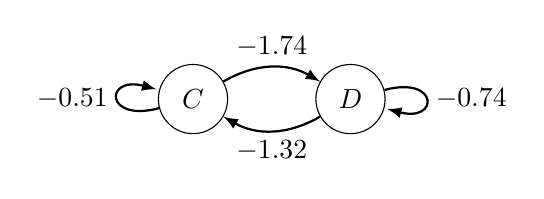
\begin{tikzpicture}[node distance=2cm,->,>=latex,auto,
  every edge/.append style={thick}]
  \node[state] (1) {$C$};
  \node[state] (2) [right of=1] {$D$};  
  \path (1) edge[loop left]  node{$-0.51$} (1)
            edge[bend left]  node{$-1.74$}   (2)
        (2) edge[loop right] node{$-0.74$}  (2)
            edge[bend left] node{$-1.32$}     (1);
\end{tikzpicture}
\end{center}
\begin{table}[h!]
\centering
\begin{tabular}{|l|l|l|}
\hline
\multicolumn{1}{|c|}{$k$} & \multicolumn{1}{c|}{$\ln{P(X_t=k\mid Y_t=C)}$} & $\ln{P(X_t=k \mid Y_t=D)}$ \\ \hline
1                           & -0.69                           & -1.21      \\ \hline
2                           & -0.91                           & -0.69         \\ \hline
3                           & -2.30                           & -1.61      \\ \hline
\end{tabular}
\end{table}

 We observed $X_1 = 1$ and $X_2 = 2$. (Note that taking the maximum of log probabilities will give you the same result as taking the maximum of probabilities as log is a monotonically increasing function.)

    
\begin{subparts}
    \subpart[1] Compute $\ln{\omega_1(C)}$ and $\ln{\omega_1(D)}$. If your answers involves decimal numbers, please round your answer to \textbf{TWO} decimal places.
    
    \textit{Note}: Showing your work in these questions is optional, but it is recommended to help us understand where any misconceptions may occur. Only your answer in the left box will be graded.
    
    What is $\ln{\omega_1(C)}$? \\
    \begin{your_solution}[title=$\ln{\omega_1(C)}$,height=2cm,width=3cm]
    % YOUR ANSWER 
    \end{your_solution}
    \begin{your_solution}[title=Work,height=4cm,width=12cm]
    % YOUR ANSWER 
    \end{your_solution}
    
    What is $\ln{\omega_1(D)}$? \\
    \begin{your_solution}[title=$\ln{\omega_1(D)}$,height=2cm,width=3cm]
    % YOUR ANSWER 
    \end{your_solution}
    \begin{your_solution}[title=Work,height=4cm,width=12cm]
    % YOUR ANSWER 
    \end{your_solution}
    
    \clearpage 
    
    \subpart[2] (\textbf{Select one}) Which of the following is the most likely sequence of hidden states? 
    
    \begin{list}{}
    % YOUR ANSWER
    % Change \emptycircle to \filledcircle for the appropriate selection/selections
        \item 
            \emptycircle
            % \filledcircle
            $Y_1=C$, $Y_2=C$ 
        \item 
            \emptycircle 
            % \filledcircle
            $Y_1=D$, $Y_2=D$ 
        \item 
            \emptycircle
            % \filledcircle
            $Y_1=D$, $Y_2=C$
        \item 
            \emptycircle
            % \filledcircle
            $Y_1=C$, $Y_2=D$ 
        \item 
            \emptycircle
            % \filledcircle
            Not enough information. 
    \end{list}
    
    
\end{subparts}
\end{parts}
\clearpage

{\Large \question Warm-up Exercise: Forward-Backward Algorithm}

\begin{parts}  \label{hmm-problem}
\part[4] To help you prepare to implement the HMM forward-backward algorithm (see Section~\ref{forback} for a detailed explanation), we have provided a small example for you to work through by hand. This toy data set consists of a training set of three sequences with three unique words and two tags and a validation set with a single sequence composed of the same unique words used in the training set. 

\textbf{Training set:}
\begin{verbatim}
you_D eat_C fish_D
you_D fish_D eat_C
eat_C fish_D
\end{verbatim}

Where the training word sequences are:
\begin{align*}
    \mathbf{x}^{(1)} &= [\texttt{you eat fish}]^T \\
    \mathbf{x}^{(2)} &= [\texttt{you fish eat}]^T \\
    \mathbf{x}^{(3)} &= [\texttt{eat fish}]^T 
\end{align*}

And the corresponding tags are:
\begin{align*}
    \mathbf{y}^{(1)} &= [D~~C~~D]^T \\
    \mathbf{y}^{(2)} &= [D~~D~~C]^T \\
    \mathbf{y}^{(3)} &= [C~~D]^T
\end{align*}

\textbf{Validation set:}
\begin{verbatim}
fish eat you
\end{verbatim}

Where the validation word sequences are: 
$$
\mathbf{x}_{\text{validation}}= 
\begin{bmatrix}
\texttt{fish eat you}\\
\end{bmatrix}^T
$$

\vspace{0.5cm}
In this question, we define
\begin{itemize}
    \item Each observed state $x_t \in \{1,2,3\}$, where 1 corresponds to \texttt{you}, 2 corresponds to \texttt{eat}, and 3 corresponds to \texttt{fish}
    \item Each hidden state $Y_t$ $\in \{C,D\}$. Let $s_1 = C$ and $s_2 = D$.
    \item $\mathbf{A}$ is the transition matrix, where $A_{jk} = P(Y_{t} = s_{k} \mid Y_{t-1} = s_{j})$. Note, here $\mathbf{A}$ is a $2 \times 2$ matrix. 
    \item $\mathbf{B}$ is the emission matrix, where $B_{jk} = P(X_{t} = k \mid Y_{t} = s_{j})$. Note, here $\mathbf{B}$ is a $2 \times 3$ matrix. As an example, $B_{23}$ denotes $P(X_{t} = 3 \mid Y_{t} = s_{2})$, or the probability $X_{t}$ corresponds to \texttt{fish} given the hidden state $Y_t = D$
    \item $\boldsymbol{\pi}$ describes $Y_1$'s initialization probabilities: $\pi_j = P(Y_1 = s_j)$
    \vspace{1.5cm}
    \item $\alpha_t(j) = P(Y_t = s_j, x_{1:t})$, which can be computed recursively:
        \begin{enumerate}
            \item $\alpha_1(j)=\pi_jB_{jx_1}$. 
            \item For $t > 1$, $\alpha_{t}(j)=B_{jx_{t}}\sum_{k=1}^{J}\alpha_{t-1}(k)A_{kj}$ 
        \end{enumerate}
    \item  $\beta_t(j) = P(x_{t+1:T} \mid Y_t = s_j)$, which can be computed recursively:
        \begin{enumerate}
            \item $\beta_T(j) = 1$ 
            \item  For $1\leq t \leq T-1$, $\beta_t(j) = \sum_{k=1}^{J}B_{kx_{t+1}}\beta_{t+1}(k)A_{jk}$ 
        \end{enumerate}
\end{itemize} 
\vspace{0.5cm}

The following four subparts are meant to encourage you to work through the forward backward algorithm by hand using this validation example. Feel free to use a calculator, being careful to carry enough significant figures through your computations to avoid rounding errors. For each subpart below, please report the requested value in the text box under the subpart (these boxes are only visible in the template document). 

\textbf{Note:} pseudo count used in section~\ref{learn} should also used here.

\textit{Note}: Showing your work in these questions is optional, but it is recommended to help us understand where any misconceptions may occur. Only your answer in the left box will be graded.

    
\begin{subparts}
    \subpart[1] Compute $\alpha_2(C)$, the $\alpha$ value associated with the tag ``C'' for the second word in the validation sequence. Please round your answer to \textbf{THREE} decimal places.
    
    \begin{your_solution}[title=$\alpha_2(C)$,height=2cm,width=3cm]
    % YOUR ANSWER 
    \end{your_solution}
    \begin{your_solution}[title=Work,height=11cm,width=13cm]
    % YOUR ANSWER 
    \end{your_solution}
    
    \clearpage
    \subpart[1] Compute $\beta_2(D)$, the $\beta$ value associated with the tag ``D'' for the second word in the validation sequence. Please round your answer to \textbf{THREE} decimal places.
    
    \begin{your_solution}[title=$\beta_2(D)$,height=2cm,width=3cm]
    % YOUR ANSWER 
    \end{your_solution}
    \begin{your_solution}[title=Work,height=5cm,width=12cm]
    % YOUR ANSWER
    \end{your_solution}    
    
    \subpart[1] Predict the tag for the third word in the validation sequence. 
    
    \begin{your_solution}[title=Tag,height=2cm,width=3cm]
    % YOUR ANSWER 
    \end{your_solution}
    \begin{your_solution}[title=Work,height=4cm,width=12cm]
    % YOUR ANSWER 
    \end{your_solution}  
    
    \subpart[1] Compute the log-likelihood for the entire validation sequence, ``\texttt{fish eat you}". Please round your answer to \textbf{THREE} decimal places.
    
    \begin{your_solution}[title=Log-Likelihood,height=2cm,width=3cm]
    % YOUR ANSWER 
    \end{your_solution}
    \begin{your_solution}[title=Work,height=4cm,width=12cm]
    % YOUR ANSWER 
    \end{your_solution} 
    
\end{subparts}

\clearpage

\part[6] Return to these subparts after implementing your \texttt{learnhmm.\{py|java|cpp\}} and \texttt{forwardbackward.\{py|java|cpp\}} functions. Please ensure that you have used the log-sum-exp trick in your programming as described in section 3.3 before answering these empirical questions.

Using the fulldata set \textbf{trainwords.txt} in the handout using your implementation of\\ \texttt{learnhmm.\{py|java|cpp\}} to learn parameters for an hmm model using the first 10, 100, 1000, and 10000 sequences in the file.
Use these learned parameters to perform prediction on the \textbf{trainwords.txt} and the \textbf{validationwords.txt} files using your \texttt{forwardbackward.\{py|java|cpp\}}.
Construct a plot with number of sequences used for training on the x-axis (log-scale) and average log likelihood across all sequences from the \textbf{trainwords.txt} and the \textbf{validationwords.txt} on the y-axis (see Section~\ref{forback} for details on computing the log data likelihood for a sequence). Each table entry is worth 0.5 points. 
Write the resulting log likelihood values in the table in the template.
Include your plot in the large box in the template (2 points).
To receive credit for your plot, you must submit a computer generated plot.
\textbf{DO NOT} hand draw your plot.


\begin{subparts}
\subpart[4] Fill in this table.

% YOUR ANSWER 
% Fill in the table by replacing the ??s with the appropriately calculated likelihood
\begin{table}[h]
    \center
    \begin{tabular}{|m{2cm}|m{3cm}|m{3cm}|}
    \hline
    \# Sequences & Train Average Log-Likelihood & Validation Average Log-Likelihood \\ \hline
    10         &  ?? & ?? \\ \hline
    100        &  ?? & ?? \\ \hline
    1000       &  ?? & ?? \\ \hline
    10000      &  ?? & ?? \\ \hline
    \end{tabular}
    \end{table}
    

\subpart[2] Put your plot below:

    \begin{your_solution}[title=$Plot$,height=10cm,width=15cm]
        % YOUR ANSWER 
        % \begin{center}
        %    \includegraphics[height8.5cm]{allplot.png}
        % \end{center}


    \end{your_solution}



\end{subparts}

\end{parts}

\clearpage
{\Large Collaboration Questions}

After you have completed all other components of this assignment, report your answers to these questions regarding the collaboration policy. Details of the policy can be found \href{https://www.cs.cmu.edu/~10601/#policies}{here}.
\begin{enumerate}
    \item Did you receive any help whatsoever from anyone in solving this assignment? Is so, include full details.
    \item Did you give any help whatsoever to anyone in solving this assignment? Is so, include full details.
    \item Did you find or come across code that implements any part of this assignment ? If so, include full details.
\end{enumerate}

\begin{your_solution}[title=Answer,height=10cm,width=15cm]
    % YOUR ANSWER 
\end{your_solution}

\clearpage\newpage
\end{questions}

{\LARGE \bf Programming (80 points)}
\label{programming}

\section{The Tasks and Data Sets}\label{dataset}
In the programming section you will implement a named entity recognition system using HMMs. Named entity recognition is the task of classifying named entities (typically proper nouns) into pre-defined categories (e.g. person, location, organization, etc). Consider the example below, where each word is appended with an underscore and then its tag:

\texttt{All-rounder\_O Phill\_PER Simmons\_PER lead\_O Somorset\_ORG in\_O win\_O}

The words \texttt{Phill} and \texttt{Simmons} are labeled as a person (\texttt{PER}), while the word \texttt{Somorset} is labeled as an organization (\texttt{ORG}). Words that aren't named entities are assigned the \texttt{O} tag.

Named entity is an incredibly important task for a machine to begin to analyze and interpret a body of natural language text. For example, when designing a system that automatically summarizes all of the day's news articles, it is important to recognize the key subjects in the articles. Another example is designing a trivia bot. If you can quickly extract the named entities from the trivia question, you may be able to more easily query your knowledge base (e.g. type a query into Google) to request information about the answer to the question.

On a technical level, the main task is to implement an algorithm to learn the hidden Markov model parameters given the training data and then implement a the forward backward algorithm to perform a smoothing query which we can then use to predict the hidden tags for a sequence of words. 

The handout files for this assignments contains several files that you will use in the homework. The contents and formatting of each of these files is explained below. 
\begin{enumerate}

\item \textbf{trainwords.txt} This file contains labeled text data that you will use in training your model in the \textbf{Learning} problem. Specifically the text contains one sentence per line that has already been preprocessed, cleaned and tokenized. You should treat every line as a separate sequence and assume that it has the following format:

    \texttt{<Word0>\_<Tag0> <Word1>\_<Tag1> ... <WordN>\_<TagN>}

where every \texttt{<WordK>\_<TagK>} unit token is separated by white space.

\item \textbf{validationwords.txt}: This file contains labeled data that you will use to evaluate your model in the \textbf{Experiments} section. This file contains the gold standard labels.  This file has the same format as \textbf{trainwords.txt}.
    
\item \textbf{index\_to\_word.txt} and \textbf{index\_to\_tag.txt}: These files contain a list of all words or tags that appear in the data set. In your functions, you will convert the string representation of words or tags to indices corresponding to the location of the word or tag in these files. For example, if Austria is on line 729 of \textbf{index\_to\_word.txt}, then all appearances of Austria in the data sets should be converted to the index 729. This index will also correspond to locations in the parameter matrices. For example, the word Austria corresponds to the parameters in column 729 of the matrix stored in \textbf{hmmemit.txt}. This will be useful for your forward-backward algorithm implementation (see Section~\ref{forback}).
    
\item \textbf{toytrain.txt}, \textbf{toyvalidation.txt}, \textbf{toy\_index\_to\_word.txt}, and \textbf{toy\_index\_to\_tag.txt}: These files are analogous to \textbf{trainwords.txt}, \textbf{validationwords.txt}, \textbf{index\_to\_word.txt}, and \textbf{index\_to\_tag.txt} and are used to compare your implementation to your hand calculations in the Written component.

\item \textbf{predictvalidation.txt} The \textbf{predictvalidation.txt} file contains labeled data that you will use to debug your implementation. The labels in this file are not gold standard but are generated by running our decoder using the features from \textbf{trainwords.txt}. This file has the same format as \textbf{trainwords.txt}.

\item \textbf{metrics.txt} The \textbf{metrics.txt} file contains the metrics you will compute for the dataset. For this assignment, you need to compute the average log likelihood and your prediction accuracy on the validation data. Note that in Named Entity Recognition, F-1 score is a more common metric to evaluate the model performance, here you only need to report your accuracy for tag prediction of each word. 

\item \textbf{hmmtrans.txt, hmmemit.txt and hmmprior.txt}: These files contain pre-trained model parameters of an HMM that you will use in testing your implementation of the \textbf{Learning} and \textbf{Evaluation and Decoding} problems. The format of the first two files are analogous and is as follows. Every line in these files consists of a conditional probability distribution. In the case of transition probabilities, this distribution corresponds to the probability of transitioning into another state, given a current state. Similarly, in the case of emission probabilities, this distribution corresponds to the probability of emitting a particular symbol, given a current state. For example, every line in \textbf{hmmtrans.txt} has the following format:
    
    \textbf{hmmtrans.txt}:\\
    \texttt{<ProbS1S1> ... <ProbS1SN>}\\
     \texttt{<ProbS2S1> ... <ProbS2SN>}...\\   
    
and every line in \textbf{hmmemit.txt} has the following format:
    
    \textbf{hmmemit.txt}:\\
    \texttt{<ProbS1Word1> ... <ProbS1WordN>}\\
     \texttt{<ProbS2Word1> ... <ProbS2WordN>}...\\
    
In both cases, elements in the same row are separated by white space. Each row corresponds to a line of text (using \texttt{\char`\\ n} to create new lines).
    
    
The format of \textbf{hmmprior.txt} is similarly defined except that it only contains a single probability distribution over starting states. Therefore each row only has a single element. Therefore \textbf{hmmprior.txt} has the following format:
    
    \textbf{hmmprior.txt}:\\
    \texttt{<ProbS1>}\\
     \texttt{<ProbS2>}...\\

\end{enumerate}

Note that the data provided to you is to help in developing your implementation of the HMM algorithms. Your code will be tested on Gradescope using different data with different HMM parameters, likely coming from a different domain although the format will be identical.

\section{Learning}\label{learn}
Your first task is to implement an algorithm to learn the hidden Markov model parameters needed to apply the forward backward algorithm (See Section \ref{forback}). There are three sets of parameters that you will need to estimate: the initialization probabilities {\boldmath$\pi$}, the transition probabilities $\mathbf A$, and the emission probabilities $\mathbf B$. For this assignment, we model each of these probabilities using a multinomial distribution with parameters $ \pi_j=P(Y_1=s_j)$, $ A_{jk} = P(Y_{t}=s_k\mid Y_{t-1}=s_j)$, and $ B_{jk} = P(X_t=k\mid Y_{t}=s_j)$. These can be estimated using maximum likelihood, which results in the following parameter estimators:

\begin{enumerate}
    \item $P(Y_1 = s_j) = \pi_j = \frac{N_{Y_1=s_j}+1}{\sum_{p=1}^{J}(N_{Y_1=s_p}+1)}$, where $N_{Y_1=s_j}$ equals the number of times state $s_j$ is associated with the first word of a sentence in the training data set.
    \item $P(Y_{t} = s_k\mid Y_{t-1}=s_j) = A_{jk}= \frac{N_{Y_t=s_k,Y_{t-1}=s_j}+1}{\sum_{p=1}^J (N_{Y_t=s_p,Y_{t-1}=s_j}+1)}$, where $N_{Y_t=s_k,Y_{t-1}=s_j}$ is the number of times state $s_j$ is followed by state $s_k$ in the training data set.  
    \item $P(X_{t} = k\mid Y_{t}=s_j) = B_{jk}= \frac{N_{X_t=k,Y_t=s_j}+1}{\sum_{p=1}^M (N_{X_t=p,Y_t=s_j}+1)}$, where $N_{X_t=k,Y_t=s_j}$ is the number of times that the state $s_j$ is associated with the word $k$ in the training data set.
\end{enumerate}

Note that for each count, a ``+1'' is added to make a \textbf{pseudocount}. This is slightly different from pure maximum likelihood estimation, but it is useful in improving performance when evaluating unseen cases during evaluation of your validation set.

You should implement a function that reads in the training data set (\textbf{trainwords.txt}), and then estimates $\pi$, $A$, and $B$ using the above maximum likelihood solutions. 

Your outputs should be in the same format as \textbf{hmmprior.txt}, \textbf{hmmtrans.txt}, and \textbf{hmmemit.txt} (including the same number of decimal places to ensure there are no rounding errors during prediction). The autograder will use the following commands to call your function:

\begin{tabbing}
For Python: \=\texttt{\$ \textbf{python} learnhmm.\textbf{py} [args\dots]}\\

For Java: \>\texttt{\$ \textbf{javac} -cp "./lib/ejml-v0.33-libs/*:./" learnhmm.\textbf{java};}\\
\>\texttt{\textbf{java} -cp "./lib/ejml-v0.33-libs/*:./" learnhmm [args\dots]}\\

For C++: \>\texttt{\$ \textbf{g++} -g -std=c++11 -I./lib learnhmm.\textbf{cpp}; ./a.out [args\dots]}\\
\end{tabbing}

Where above \texttt{[args\dots]} is a placeholder for six command-line arguments:\texttt{<train\_input>} \texttt{<index\_to\_word>} \texttt{<index\_to\_tag>} \texttt{<hmmprior>} \texttt{<hmmemit>} \texttt{<hmmtrans>}. These arguments are described in detail below:
\begin{enumerate}
    \item \texttt{<train\_input>}: path to the training input \texttt{.txt} file (see Section~\ref{dataset})
    \item \texttt{<index\_to\_word>}: path to the \texttt{.txt} that specifies the dictionary mapping from words to indices. The tags are ordered by index, with the first word having index of 1, the second word having index of 2, etc.
    \item \texttt{<index\_to\_tag>}: path to the \texttt{.txt} that specifies the dictionary mapping from tags to indices. The tags are ordered by index, with the first tag having index of 1, the second tag having index of 2, etc.
    \item \texttt{<hmmprior>}: path to output \texttt{.txt} file to which the estimated prior (\boldmath${\pi}$) will be written. The file output to this path should be in the same format as the handout \texttt{hmmprior.txt} (see Section~\ref{dataset}).
    \item \texttt{<hmmemit>}: path to output \texttt{.txt} file to which the emission probabilities ($\mathbf B$) will be written. The file output to this path should be in the same format as the handout \texttt{hmmemit.txt} (see Section~\ref{dataset})
    \item \texttt{<hmmtrans>}: path to output \texttt{.txt} file to which the transition probabilities ($\mathbf A$) will be written. The file output to this path should be in the same format as the handout \texttt{hmmtrans.txt} (see Section~\ref{dataset})..
\end{enumerate}

\newpage

\section{Evaluation and Decoding}
\label{forback}

\subsection{Forward Backward Algorithm and Minimal Bayes Risk Decoding}

Your next task is to implement the forward-backward algorithm. Suppose we have a set of sequence consisting of $T$ words, $x_1,\dots,x_T$. Each word is associated with a label $Y_t\in\{1,\dots,J\}$. In the forward-backward algorithm we seek to approximate $P(Y_t \mid x_{1:T})$ up to a multiplication constant. This is done by first breaking $P(Y_t \mid x_{1:T})$ into a ``forward'' component and a ``backward'' component as follows:
\begin{align*}
   P(Y_t =s_j \mid x_{1:T}) &\propto P(Y_t=s_j,x_{t+1:T} \mid x_{1:t})\\
   &\propto P(Y_t=s_j \mid x_{1:t})P(x_{t+1:T} \mid Y_t=s_j, x_{1:t})\\
    &\propto P(Y_t=s_j \mid x_{1:t})P(x_{t+1:T} \mid Y_t=s_j)\\ 
     &\propto P(Y_t=s_j, x_{1:t})P(x_{t+1:T} \mid Y_t=s_j) 
\end{align*}



where $P(Y_t=s_j \mid x_1,\dots,x_{t})$ is computed by passing forward recursively through the model and $P(x_{t+1},\dots,x_T \mid Y_t=s_j)$ is computed by passing recursively backwards through the model.

\textbf{Forward Algorithm}



Define $\alpha_t(j) = P(Y_t = s_j, x_{1:t})$. We can rearrange our definition of $\alpha_t(j)$ as follows:
\begin{align}
    \label{eqn:alpha}
    \alpha_t(j)
    =&P(Y_t=s_j, x_{1:t}) \nonumber\\
    =& \sum_{k} P(Y_t=s_j, Y_{t-1}=s_k, x_{1:t}) \nonumber\\
    =& \sum_{k} P(Y_{t-1}=s_k, x_{1:t} \mid Y_t = s_j) P(Y_t = s_j) \nonumber\\
    =& \sum_{k} P(x_t \mid Y_t = s_j) P(Y_{t-1}=s_k, x_{1:t-1} \mid Y_t = s_j) P(Y_t = s_j) \nonumber\\
    =& P(x_t \mid Y_t = s_j) \sum_{k} P(Y_t = s_j, Y_{t-1}=s_k, x_{1:t-1}) \nonumber\\
    =& P(x_t \mid Y_t = s_j) \sum_{k} P(Y_t = s_j, x_{1:t-1} \mid Y_{t-1}=s_k) P(Y_{t-1}=s_k) \nonumber\\
    =& P(x_t \mid Y_t = s_j) \sum_{k} P(Y_t = s_j \mid Y_{t-1}=s_k) P(x_{1:t-1} \mid Y_{t-1}=s_k) P(Y_{t-1}=s_k) \nonumber\\
    =& P(x_t \mid Y_t = s_j) \sum_{k} P(Y_t = s_j \mid Y_{t-1}=s_k) P(Y_{t-1}=s_k, x_{1:t-1}) \nonumber\\
    =& B_{jx_t} \sum_{k} A_{kj} \alpha_{t-1}(k)
\end{align}

Using this definition, the $\alpha$'s can be computed using the following recursive procedure:
\begin{enumerate}
    \item $\alpha_1(j)=\pi_jB_{jx_1}$. 
    \item For $t > 1$, $\alpha_{t}(j)=B_{jx_{t}}\sum_{k=1}^{J}\alpha_{t-1}(k)A_{kj}$ 
\end{enumerate}

\clearpage

\textbf{Backward Algorithm}
Define $\beta_t(j) = P(x_{t+1:T} \mid Y_t=s_j)$. We can rearrange our definition of $\beta_t(j)$ as follows:
\begin{align}
    \label{eqn:beta}
    \beta_t(j) &= P(x_{t+1:T} \mid Y_t=s_j)\nonumber\\
    &= \sum_{k=1}^JP(Y_{t+1}=s_k,x_{t+1:T} \mid Y_t=s_j)\nonumber\\
    &= \sum_{k=1}^JP(x_{t+1:T} \mid Y_t=s_j,Y_{t+1}=s_k)P(Y_{t+1}=s_k \mid Y_t=s_j)\nonumber\\
    &= \sum_{k=1}^JP(x_{t+1} \mid Y_{t+1}=s_k)P(x_{t+2:T} \mid Y_{t+1}=s_k)P(Y_{t+1}=s_k \mid Y_t=s_j)\nonumber\\
    &= \sum_{k=1}^J B_{kx_{t+1}}\beta_{t+1}(k)A_{jk}
\end{align}


Just like the $\alpha$'s, the $\beta$'s can also be computed using the following backward recursive procedure:

\begin{enumerate}
    \item $\beta_T(j) = 1$ (All states could be ending states)
    \item  For $1\leq t \leq T-1$, $\beta_t(j) = \sum_{k=1}^{J}B_{kx_{t+1}}\beta_{t+1}(k)A_{jk}$ (Generate $x_{t+1}$ from any state)
\end{enumerate}


\textbf{Forward-Backward Algorithm}
As stated above, the goal of the Forward-Backward algorithm is to compute $P(Y_t =s_j \mid x_{1:T})$. This can be done using the following equation:

$$P(Y_t =s_j \mid x_{1:T}) \propto P(Y_t=s_j, x_{1:t})P(x_{t+1:T} \mid Y_t=s_j) $$

After running your forward and backward passes through the sequence, you are now ready to estimate the conditional probabilities as:

$$P(Y_t \mid x_{1:t}) \propto \alpha_t\circ\beta_t$$
where $\circ$ is the element-wise product.

\textbf{Minimum Bayes Risk Prediction}
We will assign tags using the minimum Bayes risk predictor, defined for this problem as follows:

$$\hat{Y}_t = \argmax_{j\in \{1,\dots,J\}} P(Y_t = s_j \mid x_{1:T})$$

To resolve ties, select the tag that appears earlier in the \texttt{<index\_to\_tag>} input file.

\clearpage

\textbf{Computing the Log Likelihood of a Sequence}
When we compute the log likelihood of a sequence, we are interested in the computing the quantity $P(x_{1:T})$. We can rewrite this in terms of values we have already computed in the forward-backward algorithm as follows:

\begin{align*}
    \log{P(x_{1:T})} &= \log{\big(\sum_j P(x_{1:T},Y_t=s_j)\big)}\\
    &= \log{\big(\sum_j \alpha_T(j)\big)}
\end{align*}

\subsection{Implementation Details}

You should now implement your forward-backward algorithm as a program, \texttt{forwardbackward.\{py|java|cpp\}}. The program will read in validation data and the parameter files produced by \texttt{learnhmm.\{py|java|cpp\}}. The autograder will use the following commands to call your function:


\begin{tabbing}
For Python: \=\texttt{\$ \textbf{python} forwardbackward.\textbf{py} [args\dots]}\\
For Java: \>\texttt{\$ \textbf{javac} -cp "./lib/ejml-v0.33-libs/*:./" forwardbackward.\textbf{java}};\\ 
\>  \texttt{\$ \textbf{java} -cp "./lib/ejml-v0.33-libs/*:./" forwardbackward [args\dots]}\\
For C++: \>\texttt{\$ \textbf{g++} -g -std=c++11 -I./lib forwardbackward.\textbf{cpp}; ./a.out [args\dots]}\\
\end{tabbing}

Where above \texttt{[args\dots]} is a placeholder for seven command-line arguments:\texttt{<validation\_input>} \texttt{<index\_to\_word>} \texttt{<index\_to\_tag>} \texttt{<hmmprior>} \texttt{<hmmemit>} \texttt{<hmmtrans>} \texttt{<predicted\_file>} \texttt{<metric\_file>}. These arguments are described in detail below:
\begin{enumerate}
    \item \texttt{<validation\_input>}: path to the validation input \texttt{.txt} file that will be evaluated by your forward backward algorithm (see Section~\ref{dataset})
    \item \texttt{<index\_to\_word>}: path to the \texttt{.txt} that specifies the dictionary mapping from words to indices. The tags are ordered by index, with the first word having index of 1, the second word having index of 2, etc. This is the same file as was described for \texttt{learnhmm.\{py|java|cpp|m\}}.
    \item \texttt{<index\_to\_tag>}: path to the \texttt{.txt} that specifies the dictionary mapping from tags to indices. The tags are ordered by index, with the first tag having index of 1, the second tag having index of 2, etc. This is the same file as was described for \texttt{learnhmm.\{py|java|cpp|m\}}.
    \item \texttt{<hmmprior>}: path to input \texttt{.txt} file which contains the estimated prior (\boldmath${\pi}$).
    \item \texttt{<hmmemit>}: path to input \texttt{.txt} file which contains the emission probabilities ($\mathbf B$).
    \item \texttt{<hmmtrans>}: path to input \texttt{.txt} file which contains transition probabilities ($\mathbf A$).
    \item \texttt{<predicted\_file>}: path to the output \texttt{.txt} file to which the predicted tags will be written. The file should be in the same format as the \texttt{<validation\_input>} file. 
    \item \texttt{<metric\_file>}: path to the output \texttt{.txt} file to which the metrics will be written. 
\end{enumerate}

\clearpage

Example command for python users:
\begin{lstlisting}
$ python forwardbackward.py toy_data/toy_train.txt \ 
toy_data/toy_index_to_word.txt toy_data/toy_index_to_tag.txt \
toy_data/toy_hmmprior.txt toy_data/toy_hmmemit.txt \
toy_data/toy_hmmtrans.txt toy_data/toy_predicted.txt \ 
toy_data/toy_metrics.txt
\end{lstlisting}

After running the command above, the \texttt{<predicted\_file>} output should be:

\begin{lstlisting}
you_B eat_A fish_B
you_B fish_B eat_A
eat_A fish_B
\end{lstlisting}

And the \texttt{<metric\_file>} output should be:

\begin{lstlisting}
Average Log-Likelihood: -2.776793
Accuracy: 1.0
\end{lstlisting}

Take care that your output has the exact same format as shown above. There should be a single space after the colon preceding the metric value (e.g. a space after \lstinline{Average Log-Likelihood:}). Each line should be terminated by a Unix line ending \lstinline{\n}.



\subsection{Log-Space Arithmetic for Avoiding Underflow}
\label{sec:underflow}

Handling underflow properly is a critical step in implementing an HMM. And the most generalized way of handling numerical underflow due to products of small positive numbers (like probabilities) is to calculate everything in \textbf{log-space}, i.e., represent every quantity by their logarithm, 

For this homework, using log-space trick starts with transforming Eq.(\ref{eqn:alpha}) and Eq.(\ref{eqn:beta}) into logarithmic form (how to do that is straightforward and left as an exercise). Please use $e$ as the base for logarithm calculation (natural log).

After transforming the equations into log form, you may discover calculation of the following type:

$$ \log \sum_i \exp{(v_i)}$$

This may be programmed as is, but $\exp{(v_i)}$ may cause underflow when $v_i$ is large and negative. One way to avoid this is to use the \href{https://www.xarg.org/2016/06/the-log-sum-exp-trick-in-machine-learning/}{log-sum-exp trick}. We provide the pseudo code for this trick in Algorithm \ref{alg:log-sum-exp-trick}:


\begin{algorithm}[H]
    \caption{Log-Sum-Exp Trick}
    \label{alg:log-sum-exp-trick}
    \begin{algorithmic}[1]
        \Procedure{LogSumExpTrick}{($v_1, v_2, \cdots, v_n$)}
            \State $m = \max(v_i)$ for $i=\{1, 2,\cdots, n\}$ 
            \State \textbf{return }{$m + \log(\sum_i\exp(v_i-m))$} 
        \EndProcedure
    \end{algorithmic}
\end{algorithm}
\clearpage
    
\section{Gradescope Submission}

You should submit your \texttt{learnhmm.\{py|java|cpp\}} and %\newline 
\texttt{forwardbackward.\{py|java|cpp\}} to Gradescope.
Note: please do not use other file names. This will cause problems for the autograder to correctly detect and run your code.

Some additional tips: 
Make sure to read the autograder output carefully. The autograder for Gradescope prints out some additional 
information about the tests that it ran. For this programming assignment we've specially designed some buggy implementations that you might do, and try our best to detect those and give you some more useful feedback in Gradescope's autograder. Make wise use of autograder's output for debugging your code. 


Note: For this assignment, you have unlimited submissions to Gradescope before the deadline, but only your last submission will be graded.
   
    
%%%%%%%%%%%%%%%%%%%%%%%%%%%%%%%%%%%%%%%%%%%%%%%%%%%%%%%%%%%%%%%%%%%%%%%%%%%%%%%%%%%



\newpage

\end{document}